%########################################
%CS 461 CAPSTONE 
%GROUP 20 - Griffin Gonsalves, Paul Kwak, Shawn Cross
%FALL 2016
%########################################
\documentclass[letterpaper, 10pt, draftclsnofoot, compsoc, onecolumn]{IEEEtran}
\usepackage[latin1]{inputenc}
\usepackage[T1]{fontenc}
\usepackage[english]{babel}
\usepackage{amsmath}
\usepackage{amssymb,amsfonts,textcomp}
\usepackage{color}
\usepackage{array}
\usepackage{supertabular}
\usepackage{hhline}
\usepackage{color,soul}
%\usepackage{biblatex}
\usepackage{cite}


\usepackage{hyperref}
%\usepackage{digsig} %not a default package... just for signature field on final page.
\usepackage{url}

\usepackage{comment}

\hypersetup{pdftex, colorlinks=true, linkcolor=black, citecolor=blue, filecolor=blue, urlcolor=blue, pdftitle=SYSTEMS AND SOFTWARE REQUIREMENTS SPECIFICATION (SSRS) TEMPLATE, pdfauthor=Clinton Jeffery, pdfsubject=, pdfkeywords=}
\usepackage[pdftex]{graphicx}
% Outline numbering
\setcounter{secnumdepth}{4}
\renewcommand\thesection{\arabic{section}}
\renewcommand\thesubsection{\arabic{section}.\arabic{subsection}}
\renewcommand\thesubsubsection{\arabic{section}.\arabic{subsection}.\arabic{subsubsection}}
\renewcommand\theparagraph{\arabic{section}.\arabic{subsection}.\arabic{subsubsection}.\arabic{paragraph}}

\parindent0pt
\parskip 1.5ex plus 0.2ex minus 0.1ex
\makeatletter

\def\subsubsection{\@startsection{subsubsection}% name
                                 {3}% level
                                 {\z@}% indent (formerly \parindent)
                                 {1ex plus 0.1ex minus 0.1ex}% before skip
                                 {1ex}% after skip
                                 {\normalfont\normalsize}}% style

\newcommand\arraybslash{\let\\\@arraycr}
\makeatother
% Page layout (geometry)
\setlength\voffset{-1in}
\setlength\hoffset{-1in}
\setlength\topmargin{0.5in}
\setlength\oddsidemargin{.75in}
\setlength\evensidemargin{.75in}
\setlength\textheight{8.278in}
\setlength\textwidth{6.5in}
\setlength\footskip{0.561in}
\setlength\headheight{0.5in}
\setlength\headsep{0.461in}
% Footnote rule
\setlength{\skip\footins}{0.0469in}
\renewcommand\footnoterule{\vspace*{-0.0071in}\setlength\leftskip{0pt}\setlength\rightskip{0pt plus 1fil}\noindent\textcolor{black}{\rule{0.25\columnwidth}{0.0071in}}\vspace*{0.0398in}}
% Pages styles
\makeatletter
\newcommand\ps@Standard{
  \renewcommand\@oddhead{\hfill }
  \renewcommand\@evenhead{\@oddhead}
  \renewcommand\@oddfoot{\foreignlanguage{english}{\textcolor{black}{SSRS Page }}\foreignlanguage{english}{\textcolor{black}{\thepage{}}}}
  \renewcommand\@evenfoot{\@oddfoot}
  \renewcommand\thepage{\arabic{page}}
}
\newcommand\ps@FirstPage{
  \renewcommand\@oddhead{}
  \renewcommand\@evenhead{\@oddhead}
  \renewcommand\@oddfoot{}
  \renewcommand\@evenfoot{\@oddfoot}
  \renewcommand\thepage{\arabic{page}}
}
\makeatother
\pagestyle{Standard}
%\setlength\tabcolsep{1mm}
\renewcommand\arraystretch{1.3}
% footnotes configuration
\makeatletter
\renewcommand\thefootnote{\arabic{footnote}}
\makeatother
\title{Forge VR Explorer Requirements}
\author{Shawn Cross, Griffin Gonsalves, Paul Kwak}
\date{2016-11-3}


\begin{document}

\clearpage\setcounter{page}{1}\pagestyle{Standard}
\thispagestyle{FirstPage}

\bigskip

{\centering\selectlanguage{english}\bfseries\color{black}
Forge VR Explorer Design Document
\par}


\bigskip

{\centering\selectlanguage{english}\bfseries\color{black}
December 2 2016
\par}
\bigskip
\bigskip
\bigskip
\bigskip
\bigskip
\bigskip
\bigskip
\bigskip
\bigskip
\bigskip
\bigskip
\bigskip
%\begin{center}
%	
\includegraphics[scale=0.8]{forge_logo.png}
%\end{center}


\vfill
{\centering\selectlanguage{english}\bfseries\color{black}
Abstract
\par}

{\centering\selectlanguage{english}\mdseries\color{black}
	The Forge VR Explorer branches from an Autodesk prototype project called Vrok-It, which is a simple web-based 3D 
	model viewer and mobile virtual reality (VR) explorer. The project will expand upon its ability to display uploaded 3D 
	models in browser and in VR, and improve its accessibility. Conventionally, viewing 3D models in VR is a challenge if 
	you have model files on many devices, or have a headset that only works in conjunction with a smart-phone. The 
	Forge VR Explorer aims to do this by utilizing a web-based software that uses the features of the Autodesk Forge API. 
	The project will also be expanded with new ideas and stretch goals as the project is developed.
\par}
\clearpage
{\centering\selectlanguage{english}\bfseries\color{black}
TABLE OF CONTENTS
\par}

\bigskip

\setcounter{tocdepth}{2}
\renewcommand\contentsname{}
\tableofcontents

\bigskip
\clearpage


\section{Introduction}
The software implemented is a web application capable of accomplishing several tasks. The software allows for the upload of CAD files, renders them on the website using the Forge API, allows the transfer and rendering of the models onto a user's mobile device, and then has the capability to allow the user to view the models in 3D with Google Cardboard, and potentially dedicated VR devices. This document aims to delve into the design of each piece of functionality and seeks to expand its design and structure.
\subsection{Scope}
The scope of this document covers the information regarding user experience data flows, the software design description and the design structure of the software. This document does not cover specific implementation decisions or quality requirements.
\subsection{Purpose}
The purpose of this software design document is to describe the user experience flows and provide the software design description to its intended audience. Additionally, this document provides a design framework that the developers will be using in order to assess the progression of the software through its development lifespan.
\subsection{Intended audience}
The intended audience of this software design document are the developers planning and building the software, and the stakeholders who include: Autodesk's Forge team, the clients and the advisors to the developers.

\section{Definitions}
\begin{description}
	\item{CAD} Computer Aided design is software used to design and view 3D models.

	\item{CAD file} The type of files that can be uploaded to the website for viewing in the Forge viewer. 
	We will  narrow down what types of files can be used as we progress through the development process.

	\item{FORGE}~\cite{forge2016} A collection of API services provided by Autodesk that provide 3D modeling services and tools.

	\item{Forge Viewer} This is one of the APIs in Forge. It displays 3D models from CAD files and also allows
	for user interaction.
	
	\item{Model Derivative API} This is another API in Forge. It can generate SVF files that we can utilize in the application from other model filetypes.
	
	\item{VR} Acronym for virtual reality, typically a peripheral device or smartphone
	\item{exploding model} A model viewing functionality that separates components from their original locations in order to gain an alternate view of the model.
\end{description} 

\subsubsection{Influences on SDD preparation}
The SRS is the main influence on the SDD as it holds the requirements and features determined necessary by all the stakeholders. This drives the design to meet those requirements to properly satisfy all stakeholders. However, this also means that it sets the design constraints.

\subsubsection{Design verification and design role validation}
In order to verify that our software meets requirements, test cases will be used in order to walkthrough the system and demonstrate the actual funtionality of the software system. In terms of user experience the verification and validation will be mainly done through some primary tests with Autodesk with final okay coming from the clients.

\subsection{Design stakeholders and their concerns}
	The primary stakeholder for this project is Patti Vrobel who works for autodesk. User experience is a primary focus of both Patti and Autodesk, and serves as an overarching goal for the project. The project addresses this by adding and altering features to make the website more accessible for users.

\section{Design Views}

\subsection{Viewable Model}
The user must be able to see the model they uploaded from the cad file. This is accomplished by using the Forge Large Model Viewer, or Forge Viewer. The model must be able to be manipulated and explored with simple and intuitive controls. This includes both a viewer on a desktop machine as well as a separate viewer exclusively for the smartphone. Because this viewer is responsible for a large aspect of the project, ensuring the viewer is configured to run as smoothly as possible is essential.

\subsection{Interface Viewpoint}
\begin{itemize}
	\item[]\textbf{Main Viewer Window} By default, there will be at least one viewer within the desktop website after a completed their file upload. This includes the Viewer Controls component.
	\item[]\textbf{Viewer Controls} The viewer is interacted with by using the Large Model Viewer's API, which is a small set of controls in a compact interface that appears at the bottom of the viewer. This set of controls can rotate, zoom, explode, or toggle settings for viewing the model. If a keyboard is connected, then a set of keys can be used to control the viewer in a basic and straightforward manner.
	\item[]\textbf{Secondary Viewer}  The Main Viewer must control a separate instance of the Viewer that runs exclusively for the connected smartphone, and matches the exact position and viewing of the desktop viewer. The main viewer is also responsible for handling the controls for the second viewer. These viewers are hosted within the web page.
	\hl{sessions?}
	\item[]\textbf{Information and Other Site Content} The website will eventually come to encompass more content as the project progresses in development. These changes will be noted in blogs, and will be made visible on the project website. These additions to the site will most likely come as feature updates to previously described components or new features on new pages of the site.
	\item[]\textbf{} 
\end{itemize}
\subsection{Rationale}

%placeholder
\begin{comment}


\subsection{Interface Viewpoint}
\begin{itemize}
	\item[]\textbf{} 
	\item[]\textbf{} 
	\item[]\textbf{}  
	\item[]\textbf{}
	\item[]\textbf{} 
\end{itemize}
\end{comment}


\subsection{Website Structure}
Because the website is the focus of the project, we are hosting a new version of the website utilizing a github project page for hosting. The requirements for the website are to properly host, arrange and display all of the components of the project. This includes the file uploading, authentication, the forge viewer, and mobile device connection software. The website must be simple to use, and appears intuitive for all users.
\subsection{Interface Viewpoint}
\begin{itemize}
	\item[]\textbf{Forge Viewer} Implementing the Forge Viewer into the page will involve calling the API within a script on the main page. The individual required files for the viewer are held in the site source files.
	\item[]\textbf{File Upload} The file upload functionality will be available on the main page in a specific area.
	\item[]\textbf{Smartphone QR Code}  The smartphone QR code will also have its own page section and will be viewable on the main page of the site.
	\item[]\textbf{}
	\item[]\textbf{} 
\end{itemize}


\subsection{Local File Upload}
	The user should be able to upload their own CAD files from a local storage device that they have access to. This will be some sort of button that is easily identifiable by the user that once selected will allow the user to browse through the local files on the current machine and select the CAD file that they would like to view. Once the file is selected the website should verify that the file is an allowed CAD drawing file. If the file is of the correct file type then the file should be converted to the SVF file type that is used by the forge viewer api. The user should be notified that the file was successfully uploaded to the website and the model that was in the file should be displayed in the list of choose-able models as well as displayed in the viewer. 

\subsection{Interface Viewpoint}
\begin{itemize}
	\item[]\textbf{Local Upload Button} There will be a button on the website for uploading files from local storage on the users machine. This button should be easy for the user to identify. Once the user has pressed the button then the user should have access to the local files on their machine.
	\item[]\textbf{File selection} The user should be able to then navigate through their local files to find the CAD file that they are wanting to view.
	\item[]\textbf{File type verification} Once a file has been selected by the user the website should verify that the file is actually usable. This should be done by checking that if the file is a CAD drawing file type that can be converted into an SVF file that is used by the viewer. If the file is a usable file then the website 			should simply proceed and convert the file. If the file is not the correct file type then the user should be notified of this and prompted to select a different file.  
	\item[]\textbf{File size verification} Large file may not work well in the viewer in this case the website should determine if a file is to large for the viewer to handle. If the file the user has selected is to large then the user should be notified that the selected file is to large and be prompted to select a different file.
	This can be done at the same time as verifying the file size.
	\item[]\textbf{File conversion} The file conversion will be done through the use of the forge model derivative api. If the conversion request was successful then the file should be added to the current list of viewable models and also placed in the viewer. If the conversion request is unsuccessful then the user should
	 be notified that their file could not be converted. 
\end{itemize}

The design constraints require that the user has the file that they are wanting to use on the current machine that they are using. They will also only be able use CAD drawing file when uploading a file to the website.  

\begin{flushleft}
	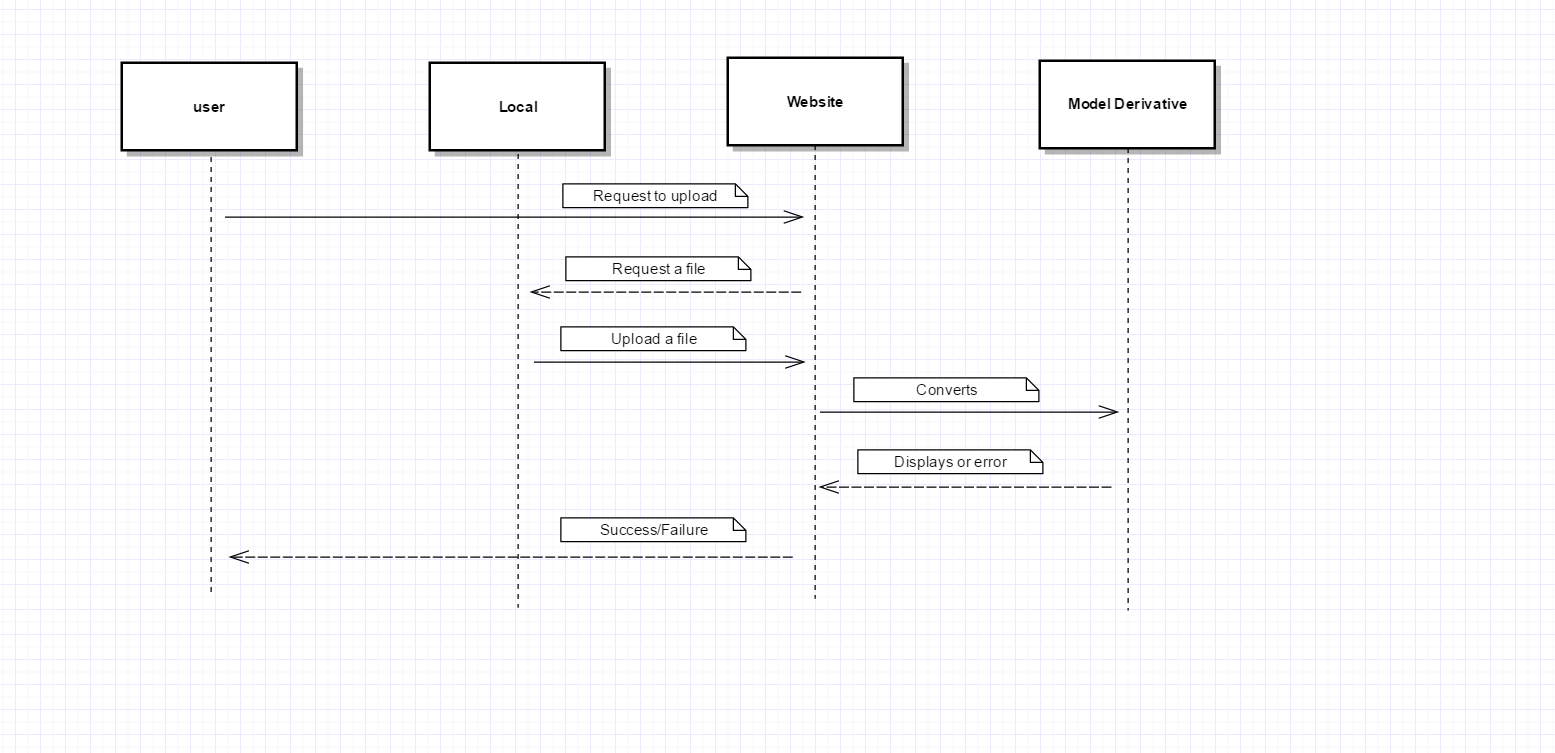
\includegraphics[scale=0.6]{localUpload.png}
\end{flushleft}

\subsection{Non-local File Upload}
	The user should be able to  access their files that are on an outside storage device and then upload these files to the website. There should be a button that the user can use to login to there outside storage. once logged in the user should be able to navigate to the file that they would like to use and then select that file to be uploaded. The website should verify that the selected file is of the correct file type and size. The website should also convert the file to an SVF file that the viewer can use. If for any reason there is a failure in the file upload then the user should be notified of that failure and informed of what to do.

\subsection{Interface Viewpoint}
\begin{itemize}
	\item[]\textbf{Non-Local Upload Button} This button should be easy for the user to identify in the main area of the web page. Once the user has pressed the button they should be prompted to login to the Autodesk account that they are trying to access.
	\item[]\textbf{User login} Using the data management api the user will be asked to login to there Autodesk account to receive an authentication token. Once logged in the user will have access to any of there Autodesk storage systems. 
	\item[]\textbf{File type verification} Once a file has been sent to the website from the outside storage should, it verify that the file is actually usable. This should be done by checking that if the file is a CAD drawing file type that can be converted into an SVF file that is used by the viewer. If the file is a usable file then the 	
	website should simply proceed and convert the file. If the file is not the correct file type then the user should be notified of this and prompted to select a different file.  
	\item[]\textbf{File selection} After the user has access they should then be able to navigate to the correct storage system their file is in and gain access to their files. Once a file is selected it should then be returned to the website. If returning the file is unsuccessful then the user should be notified and prompted to try 
	again.
	\item[]\textbf{File size verification} Large file may not work well in the viewer, in this case the website should determine if a file is to large for the viewer to handle. If the file the user has selected is to large then the user should be 		
	notified that the selected file is to large and be prompted to select a different file.
	\item[]\textbf{File conversion} The file conversion will be done through the use of the forge model derivative api. If the conversion request was successful then the file should be added to the current list of viewable models and also placed in the viewer. If the conversion request is unsuccessful then the user should
	 be notified that their file could not be converted. 
\end{itemize}
  
the design constraints require that the file or file that the user is wanting to upload be located in the outside storage that they are wanting to use. They will also only be able use CAD drawing file when uploading a file to the website.  

\begin{flushleft}
	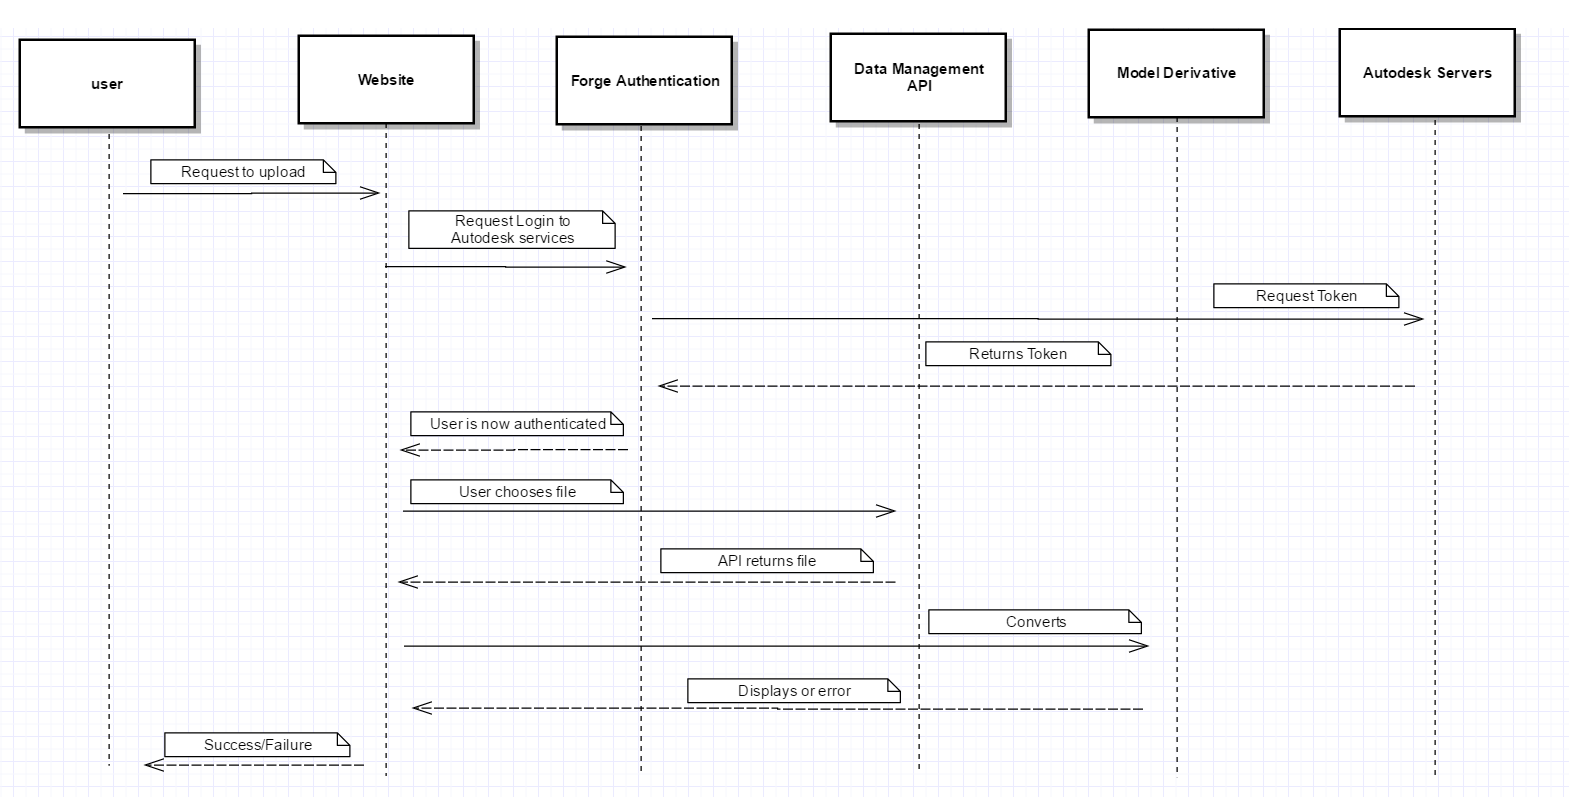
\includegraphics[scale=0.5]{nonLocalUpload.png}
\end{flushleft}

\subsection{Mobile Device Connection}
	The user should be able to connect their mobile device to the websites current session through the use of a QR code on the web page. The user will need to have a some way to scan the QR code with their mobile device. 

\subsection{Interface viewpoint}
\begin{description}
	\item\textbf{QR code} There should be a QR code generated at the beginning of every session on the web page. This will be done through the use of a jquery plug-in that generates QR codes. This plug-in can be found at \href{https://github.com/jeromeetienne/jquery-qrcode}{https://github.com/jeromeetienne/jquery-qrcode}. The QR code should be somewhere on the web page that is easy for the user to find. 
	\item\textbf{QR scanner} The user will need to have a way to scan the QR code. This will most likely be done through the use of an application on the users phone that will use there camera to scan the QR code.
	\item\textbf{Device connection} Once the user has successfully scanned the QR code their device should notify them that they are being connected to the current session. If there is any reason that the device could not connect to the session then the user should be notified that the connection has failed and advise them to try to connect again.
	\item\textbf{Device View} After the device has successfully connected to the current session then the user should see the exact same thing that is currently being displayed in the viewer. It should look as though there is two of the same images on the screen, this is for the use of viewing the object in a VR environment.  
\end{description}

\bibliography{bibfile}
\bibliographystyle{IEEETran}
\end{document}


%@misc{a javascript library for building user interfaces - react,
 %title={A JavaScript library for building user interfaces - React},
 %url={https://facebook.github.io/react/},
 %journal={A JavaScript library for building user interfaces - React}, 
 %publisher={Facebook.com}}

